% Options for packages loaded elsewhere
\PassOptionsToPackage{unicode}{hyperref}
\PassOptionsToPackage{hyphens}{url}
\PassOptionsToPackage{dvipsnames,svgnames,x11names}{xcolor}
%
\documentclass[
  letterpaper,
  DIV=11,
  numbers=noendperiod]{scrartcl}

\usepackage{amsmath,amssymb}
\usepackage{iftex}
\ifPDFTeX
  \usepackage[T1]{fontenc}
  \usepackage[utf8]{inputenc}
  \usepackage{textcomp} % provide euro and other symbols
\else % if luatex or xetex
  \usepackage{unicode-math}
  \defaultfontfeatures{Scale=MatchLowercase}
  \defaultfontfeatures[\rmfamily]{Ligatures=TeX,Scale=1}
\fi
\usepackage{lmodern}
\ifPDFTeX\else  
    % xetex/luatex font selection
\fi
% Use upquote if available, for straight quotes in verbatim environments
\IfFileExists{upquote.sty}{\usepackage{upquote}}{}
\IfFileExists{microtype.sty}{% use microtype if available
  \usepackage[]{microtype}
  \UseMicrotypeSet[protrusion]{basicmath} % disable protrusion for tt fonts
}{}
\makeatletter
\@ifundefined{KOMAClassName}{% if non-KOMA class
  \IfFileExists{parskip.sty}{%
    \usepackage{parskip}
  }{% else
    \setlength{\parindent}{0pt}
    \setlength{\parskip}{6pt plus 2pt minus 1pt}}
}{% if KOMA class
  \KOMAoptions{parskip=half}}
\makeatother
\usepackage{xcolor}
\setlength{\emergencystretch}{3em} % prevent overfull lines
\setcounter{secnumdepth}{-\maxdimen} % remove section numbering
% Make \paragraph and \subparagraph free-standing
\makeatletter
\ifx\paragraph\undefined\else
  \let\oldparagraph\paragraph
  \renewcommand{\paragraph}{
    \@ifstar
      \xxxParagraphStar
      \xxxParagraphNoStar
  }
  \newcommand{\xxxParagraphStar}[1]{\oldparagraph*{#1}\mbox{}}
  \newcommand{\xxxParagraphNoStar}[1]{\oldparagraph{#1}\mbox{}}
\fi
\ifx\subparagraph\undefined\else
  \let\oldsubparagraph\subparagraph
  \renewcommand{\subparagraph}{
    \@ifstar
      \xxxSubParagraphStar
      \xxxSubParagraphNoStar
  }
  \newcommand{\xxxSubParagraphStar}[1]{\oldsubparagraph*{#1}\mbox{}}
  \newcommand{\xxxSubParagraphNoStar}[1]{\oldsubparagraph{#1}\mbox{}}
\fi
\makeatother


\providecommand{\tightlist}{%
  \setlength{\itemsep}{0pt}\setlength{\parskip}{0pt}}\usepackage{longtable,booktabs,array}
\usepackage{calc} % for calculating minipage widths
% Correct order of tables after \paragraph or \subparagraph
\usepackage{etoolbox}
\makeatletter
\patchcmd\longtable{\par}{\if@noskipsec\mbox{}\fi\par}{}{}
\makeatother
% Allow footnotes in longtable head/foot
\IfFileExists{footnotehyper.sty}{\usepackage{footnotehyper}}{\usepackage{footnote}}
\makesavenoteenv{longtable}
\usepackage{graphicx}
\makeatletter
\newsavebox\pandoc@box
\newcommand*\pandocbounded[1]{% scales image to fit in text height/width
  \sbox\pandoc@box{#1}%
  \Gscale@div\@tempa{\textheight}{\dimexpr\ht\pandoc@box+\dp\pandoc@box\relax}%
  \Gscale@div\@tempb{\linewidth}{\wd\pandoc@box}%
  \ifdim\@tempb\p@<\@tempa\p@\let\@tempa\@tempb\fi% select the smaller of both
  \ifdim\@tempa\p@<\p@\scalebox{\@tempa}{\usebox\pandoc@box}%
  \else\usebox{\pandoc@box}%
  \fi%
}
% Set default figure placement to htbp
\def\fps@figure{htbp}
\makeatother

\KOMAoption{captions}{tableheading}
\makeatletter
\@ifpackageloaded{caption}{}{\usepackage{caption}}
\AtBeginDocument{%
\ifdefined\contentsname
  \renewcommand*\contentsname{Tabla de contenidos}
\else
  \newcommand\contentsname{Tabla de contenidos}
\fi
\ifdefined\listfigurename
  \renewcommand*\listfigurename{Listado de Figuras}
\else
  \newcommand\listfigurename{Listado de Figuras}
\fi
\ifdefined\listtablename
  \renewcommand*\listtablename{Listado de Tablas}
\else
  \newcommand\listtablename{Listado de Tablas}
\fi
\ifdefined\figurename
  \renewcommand*\figurename{Figura}
\else
  \newcommand\figurename{Figura}
\fi
\ifdefined\tablename
  \renewcommand*\tablename{Tabla}
\else
  \newcommand\tablename{Tabla}
\fi
}
\@ifpackageloaded{float}{}{\usepackage{float}}
\floatstyle{ruled}
\@ifundefined{c@chapter}{\newfloat{codelisting}{h}{lop}}{\newfloat{codelisting}{h}{lop}[chapter]}
\floatname{codelisting}{Listado}
\newcommand*\listoflistings{\listof{codelisting}{Listado de Listados}}
\makeatother
\makeatletter
\makeatother
\makeatletter
\@ifpackageloaded{caption}{}{\usepackage{caption}}
\@ifpackageloaded{subcaption}{}{\usepackage{subcaption}}
\makeatother

\ifLuaTeX
\usepackage[bidi=basic]{babel}
\else
\usepackage[bidi=default]{babel}
\fi
\babelprovide[main,import]{spanish}
% get rid of language-specific shorthands (see #6817):
\let\LanguageShortHands\languageshorthands
\def\languageshorthands#1{}
\usepackage{bookmark}

\IfFileExists{xurl.sty}{\usepackage{xurl}}{} % add URL line breaks if available
\urlstyle{same} % disable monospaced font for URLs
\hypersetup{
  pdftitle={Documentación SVAR51},
  pdflang={es},
  colorlinks=true,
  linkcolor={blue},
  filecolor={Maroon},
  citecolor={Blue},
  urlcolor={Blue},
  pdfcreator={LaTeX via pandoc}}


\title{Documentación SVAR51}
\author{}
\date{}

\begin{document}
\maketitle


\subsection{Motivación}\label{motivaciuxf3n}

La razón por la cual se planteo la creación de una variante del
\textbf{SVAR50\_5B} es debido a que existen diferencias que causan un
grado de incompatiblidad entre dicho modelo y el \textbf{QPM}. La
primera fuente de incompatibilidad proviende del hecho de que los datos
trimestrales usados en los corrimientos no son los mismos datos
trimestrales usando en el modelo QPM. Esto es algo que se observa de
forma evidente si se observan los pronósticos del Índice de precios de
transables (IPEI).

\textbf{Pronósticos SVAR50 -corrimiento mayo 2025-}

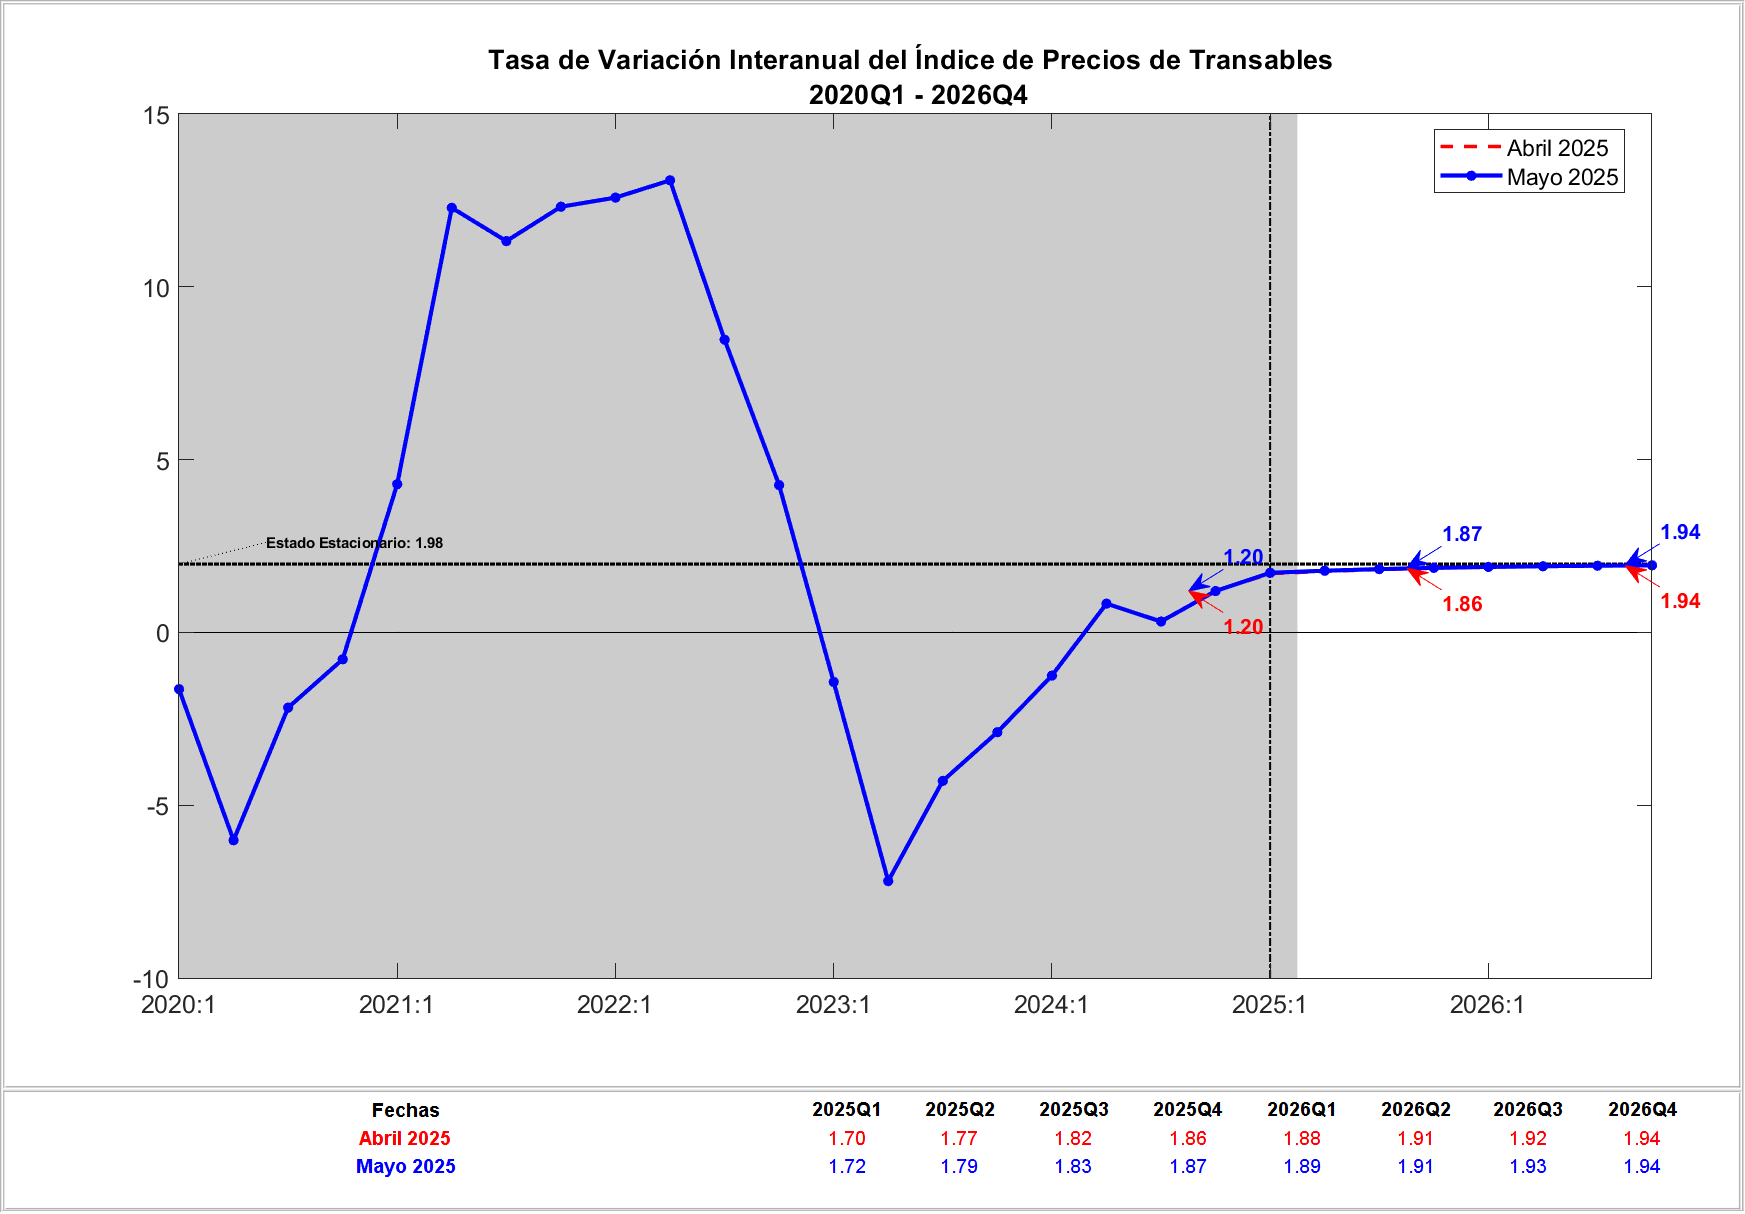
\includegraphics[width=9.375in,height=\textheight,keepaspectratio]{plots/d4_ln_ipei_short.png}

\textbf{Pronósticos QPM -corrimiento mayo 2025-}
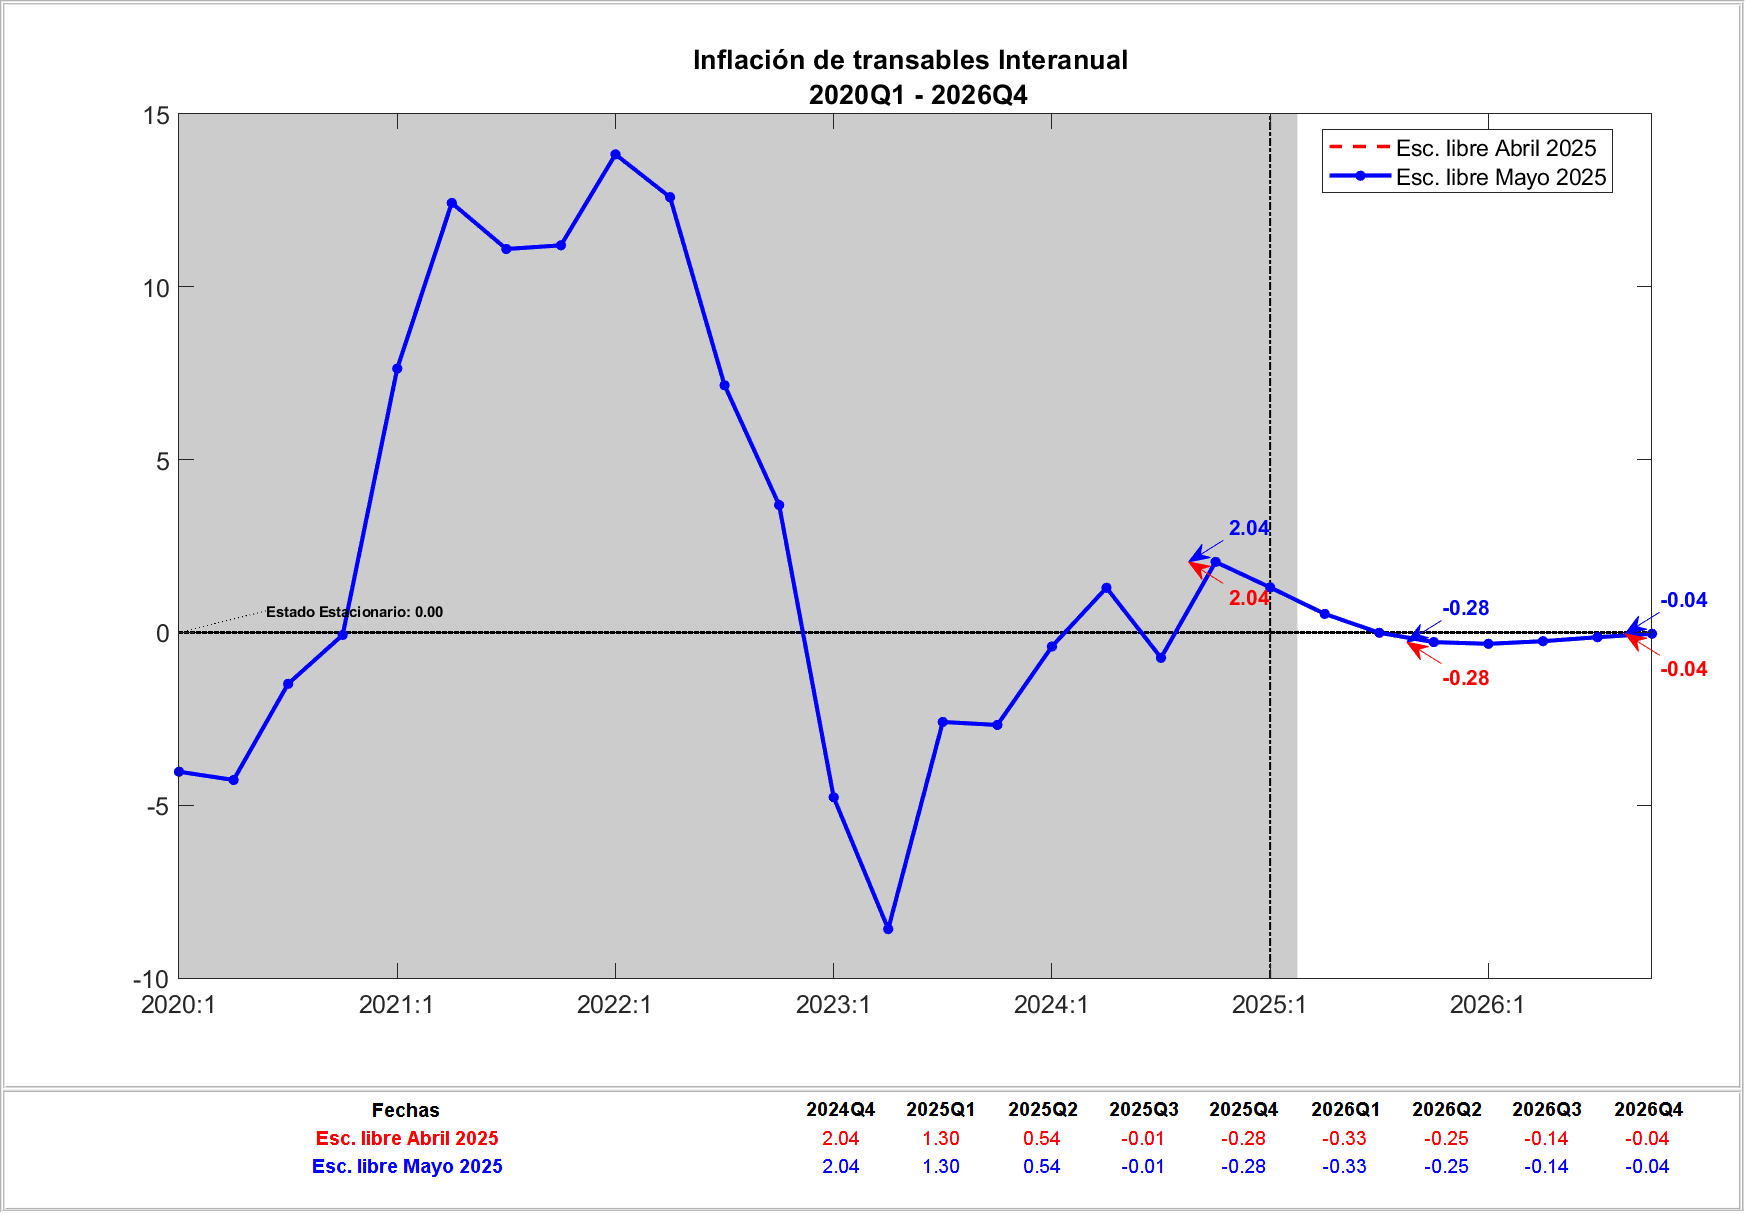
\includegraphics[width=9.375in,height=\textheight,keepaspectratio]{plots/D4L_IPEI_short.png}

La razón de ello se debe a que esta variable presenta una gran
volatilidad de un mes a otro, algo que no es capaz de capturar el
SVAR50\_4B debido a que el método de trimestralización utilizado para
este modelo es el promedio de los datos durante trimestre, en
comparación con el QPM que es el último valor observado durante el
trimestre.

Otra fuente de incompatibilidad proviene de los estados estacionarios de
algúnas variables que son de interés al momento de observar sus
pronósticos en cada corrimiento. Como se observó en las gráficas el IPEI
posee un estado estacionario de 1.98 en el SVAR50\_4B mientras que en el
QPM es de 0. Diferencias que comparten variables como inflación total,
subyacente y no subyacente.\footnote{La selección de esta variables
  corresponde a la importancia que tienen tanto para el Banco Central
  como dentro de los modelos SVAR50\_4B y QPM.}

Las fuentes de incompatbilidad se pueden dividir en dos, las que están
relacionadas con los datos y aquellas que corresponden al valor de
estado estacionario de variables de interés. A continuación se presenta
un resumen de las mismas:

\begin{table}

\caption{\label{tbl-panel}: Fuentes de incompatibilidades}

\begin{minipage}{0.50\linewidth}

\begin{longtable}[]{@{}
  >{\raggedright\arraybackslash}p{(\linewidth - 2\tabcolsep) * \real{0.4000}}
  >{\raggedright\arraybackslash}p{(\linewidth - 2\tabcolsep) * \real{0.6000}}@{}}
\caption{Datos}\tabularnewline
\toprule\noalign{}
\begin{minipage}[b]{\linewidth}\raggedright
SVAR50\_4B
\end{minipage} & \begin{minipage}[b]{\linewidth}\raggedright
QPM
\end{minipage} \\
\midrule\noalign{}
\endfirsthead
\toprule\noalign{}
\begin{minipage}[b]{\linewidth}\raggedright
SVAR50\_4B
\end{minipage} & \begin{minipage}[b]{\linewidth}\raggedright
QPM
\end{minipage} \\
\midrule\noalign{}
\endhead
\bottomrule\noalign{}
\endlastfoot
Método de trimestralización: Promedio dentro del trimestres & Método de
trimestralización: último valor observado dentro del trimestre \\
\end{longtable}

\end{minipage}%
%
\begin{minipage}{0.50\linewidth}

\begin{longtable}[]{@{}ll@{}}
\caption{Estados estacionarios}\tabularnewline
\toprule\noalign{}
SVAR50\_4B & QPM \\
\midrule\noalign{}
\endfirsthead
\toprule\noalign{}
SVAR50\_4B & QPM \\
\midrule\noalign{}
\endhead
\bottomrule\noalign{}
\endlastfoot
IPEI = 1.98 & IPEI = 0 \\
Inflación total = 4.98 & Inflación total = 4 \\
Inflación subyacente = 4.49 & Inflación subyacente = 4 \\
Inflación no subyacente = 0.44 & Inflación no subyacente = 0 \\
\end{longtable}

\end{minipage}%

\end{table}%

Por lo anterior se procedió a estimar un nuevo modelo SVAR que tuviera
como propósito subsanar las incompatibilidades entre el SVAR50\_4B y el
QPM, dicho modelo fué denominado \textbf{SVAR51} el cual es una variante
del SVAR50\_4B que comparte con este las mimas varialbes, restricciones
en la matriz de coeficientes y método de estimación, pero cambiando los
datos usados para su estimación, por lo que el modelo se estimó con
datos trimestrales cuyo método de trimestralización es el \emph{mismo
que el QPM} además de imponer los estados estacionarios de las variables
antes mencionadas de la misma forma que se encuentran en el QPM.

\subsection{Resultados de la
evaluación}\label{resultados-de-la-evaluaciuxf3n}

Utilizando la metodología de selección y evaluaicón de modelos tipo SVAR
se realizó un comparativo entre el SVAR51 y SVAR50\_4B con el propósito
de evaluar la capacidad explicativa y predictiva de la nueva variante
del SVAR50\_4B.

\subsubsection{Capacidad predictiva}\label{capacidad-predictiva}

Para un horizonte de evaluación de 10 horizontes (el mismo se utilizó
para la capacidad predictiva) y para el promedio de las 4 variables
objetivo, el SVAR51 presenta valores más altos de la métrica de
disperción comparado con el SVAR50\_4B. Lo cual lo vuelve un modelo con
mayor dispersión




\end{document}
